\documentclass{article}
\usepackage[utf8]{inputenc}
\usepackage{indentfirst}
\usepackage{titling}
\usepackage{geometry}
\usepackage{graphicx}
\usepackage{amsfonts}
\usepackage{mathtools}
\graphicspath{ {./img/} }
\usepackage[shortlabels]{enumitem}
\usepackage{fancyhdr}
\usepackage{ulem}
\usepackage[dvipsnames]{xcolor}


\renewcommand\maketitlehooka{\null\mbox{}\vfill} %para centralizar verticalmente
\renewcommand\maketitlehookd{\vfill\null}
\pagestyle{fancy}
\fancyhf{}
\rfoot{\thepage}
\lfoot{ 
\includegraphics[scale=0.01]{UA.jpg} José Mendes 107188 LEI}
\geometry{
  a4paper,
  headheight=4cm,
  top=5.5cm,
  bottom=4.5cm,
  footskip=4cm
}


\title{Compiladores}
\author{José Mendes 107188}
\date{2023}

\begin{document}


\begin{titlepage}
    \maketitle
    \begin{center}
        
\includegraphics[scale=0.4]{UA.png}
    \end{center}
    \thispagestyle{empty} %remove o count da pagina
\end{titlepage}

\pagebreak
%depois por um index aqui

\section{Tema 1 - Compiladores, Linguagens e
Gramáticas}

\subsection{Enquadramento}

\subsubsection{Linguagens}

Uma Linguagem pode definir-se pelas características:
\begin{enumerate}
  \item Permite expressar, transmitir e receber ideias;
  \item Comunicação entre pessoas ou seres vivos em geral;
  \item Inclui a comunicação com e entre máquinas;
  \item Requer várias entidades comunicantes, um código e regras para tornar a
  comunicação inteligível (isto é conjunto de regras comuns que os interlocutores reconheçam);
\end{enumerate}

\begin{flushleft}
  \item Diferentes linguagens podem ter um mesmo significado para diferentes palavras e entre estas podem ter mais do que um significado.
  \item É necessário decidir se uma sequência de símbolos do alfabeto é válida.
  \item Só sequências válidas é que permitem comunicação
  \item A comunicação pode ter um efeito, sendo esta uma resposta ou o despoletar de ações.
\end{flushleft}

\subsubsection{Linguagens de Programação}

\begin{flushleft}
  \item Partilham as características das "Linguagens Naturais".
  \item Diferem no facto de não poderem ter \textbf{ambiguidade}.
  \item Ações despoletadas podem ser mudanças do estado computacional podendo estes estar ligado a entidades externas (como outros computadores, pessoas, \dots).
  \item Podemos defini-las por estruturas formais bem comportadas. 
\end{flushleft}

\begin{flushleft}
  \textbf{Nota:} Desenvolvimento das linguagens de programação umbilicalmente ligado com as tecnologias de compilação!
\end{flushleft}

\subsection{Compiladores - Introdução}

\begin{flushleft}
  \textbf{Compiladores -} Compreensão, interpretação e/ou tradução automática de
  linguagens.
\end{flushleft}

\subsubsection{Processadores de Linguagens}

Compiladores são programas que permitem:
\begin{enumerate}
  \item Decidir sobre a correção de sequências de símbolos do
  respetivo alfabeto;
  \item Despoletar acções resultantes dessas decisões.
\end{enumerate}

\pagebreak

Frequentemente "limitam-se" a fazer a tradução entre linguagens.

\begin{center}
  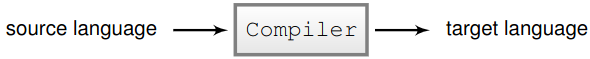
\includegraphics[scale=0.4]{1}
\end{center}

\begin{flushleft}
  \textbf{Nota:} É o caso dos compiladores das linguagens de
  programação de alto nível (Java, C++, Eiffel, etc.), que
  traduzem o código fonte dessas linguagens em código de
  linguagens mais próximas do hardware do sistema
  computacional (e.g. assembly ou Java bytecode).
\end{flushleft}

\begin{flushleft}
  \textbf{Nota:} Nestes casos, na inexistência de erros, é gerado um
  programa composto por código executável direta ou
  indiretamente pelo sistema computacional:
\end{flushleft}

\begin{center}
  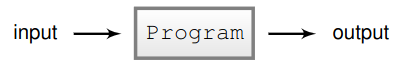
\includegraphics[scale=0.4]{2}
\end{center}

\begin{flushleft}
  \textcolor{Blue}{Exemplo:}
\end{flushleft}

\begin{center}
  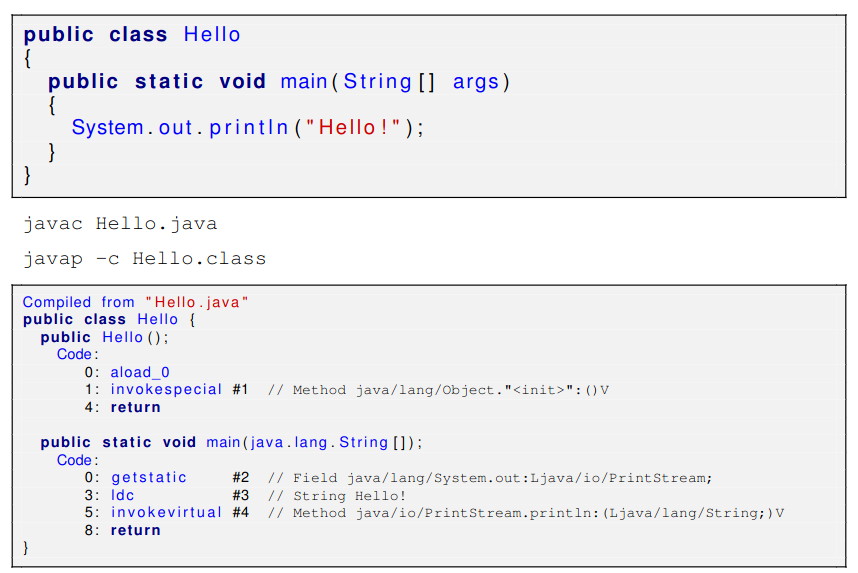
\includegraphics[scale=0.3]{3}
\end{center}

\begin{center}
  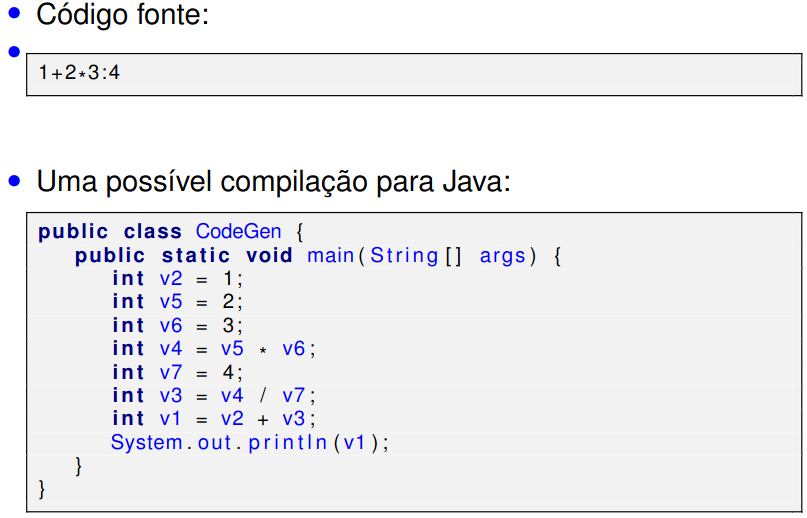
\includegraphics[scale=0.3]{4}
\end{center}

\pagebreak

\subsubsection{Interpretadores}

\begin{center}
  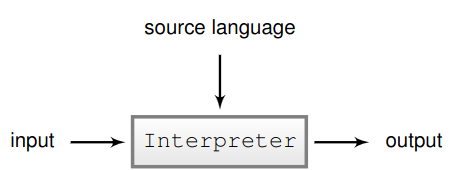
\includegraphics[scale=0.4]{5}
\end{center}

\begin{flushleft}
  \item São uma possível variante.
  \item Neste caso a execução é feita instrução a instrução (ex: python, bash, \dots).
  \item Existem também aproximações hibridas em que existe
  compilação de código para uma linguagem intermédia,
  que depois é interpretada na execução.
  \item A linguagem Java utiliza uma estratégia deste género em
  que o código fonte é compilado para Java bytecode, que
  depois é interpretado pela máquina virtual Java.
\end{flushleft}

\begin{flushleft}
  \textbf{Nota:} Em geral os compiladores processam código fonte em
  formato de texto, havendo uma grande variedade no
  formato do código gerado (texto, binário, interpretado, \dots ).
\end{flushleft}

\begin{center}
  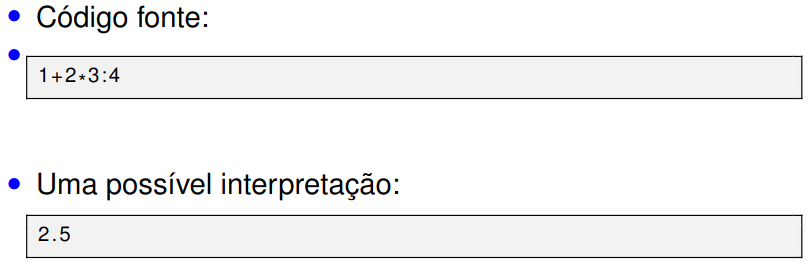
\includegraphics[scale=0.3]{6}
\end{center}

\subsection{Estrutura de um Compilador}

\begin{center}
  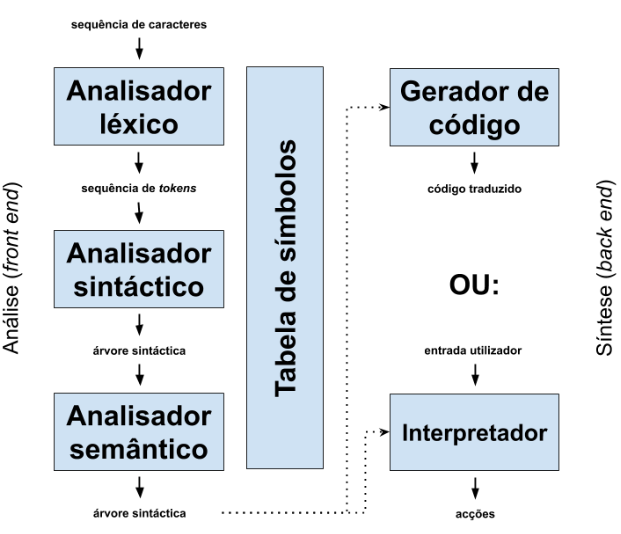
\includegraphics[scale=0.4]{7}
\end{center}

Uma característica interessante da compilação de
linguagens de alto nível, é o facto de, tal como no caso
das linguagens naturais, essa compilação envolver \textbf{mais
do que uma linguagem}:

\begin{itemize}
  \item \textbf{Análise Léxica:} composição de letras e outros caracteres
  em palavras (tokens);
  \item \textbf{Análise Sintática:} composição de tokens numa estrutura
  sintática adequada;
  \item \textbf{Análise Semântica:} verificação se a estrutura sintática
  tem significado.
\end{itemize}

As ações consistem na geração do programa na linguagem destino e podem envolver
também diferentes fases de geração de código e otimização.

\subsubsection{Análise Lexical}

\begin{flushleft}
  \item Conversão da sequência de caracteres de entrada numa
  sequência de elementos lexicais.
  \item Simplifica brutalmente a gramática da análise sintática e permite uma
  implementação mais eficiente do analisador léxico.
  \item Cada elemento lexical pode ser definido por um tuplo com uma identificação
  do elemento e do seu valor (podendo ser omitido quando N/A).
\end{flushleft}

\begin{center}
  \textbf{$<$ token\_name, attribute\_value $>$}
\end{center}

\begin{flushleft}
  \textcolor{Blue}{Exemplo:} \break

  \textbf{pos $=$ pos $+$ vel $*$ 5;}

  \vspace{3mm}

  pode ser convertido pelo analisador léxico (scanner ) em:
  
  \textcolor{BrickRed}{$< i d , pos> <=> < i d , pos> <+> < i d , v e l > <*> < i n t ,5 > <; >$}
\end{flushleft}

\begin{flushleft}
  \textbf{Nota:} Em geral os espaços em branco, e as mudanças de linha
  e os comentários não são relevantes nas linguagens de
  programação, pelo que podem ser eliminados pelo
  analisador lexical.
\end{flushleft}

\begin{flushleft}
  \textcolor{Blue}{Exemplo:} \break

  \textbf{distance ( 0 , 0 ) ( 4 , 3 )}

  \vspace{3mm}

  pode ser convertido pelo analisador léxico (scanner ) em:
  
  \textcolor{BrickRed}{$< d i s t a n c e > <(> <num,0 > <,> <num,0 > <)>
  <(> <num,4 > <,> <num,3 > <)>$}
\end{flushleft}

\pagebreak

\subsubsection{Análise Sintática}

\begin{flushleft}
  \item Após a análise lexical segue-se a chamada análise
  sintática (\textbf{parsing}), onde se verifica a conformidade da
  sequência de elementos lexicais (\textbf{tokens}) com a estrutura
  sintática da linguagem.
  \item Nas linguagens que se pretende sintaticamente
  processar, podemos sempre fazer uma aproximação à sua
  estrutura formal através duma representação tipo árvore (\textbf{árvore sintática}).
  \item Para esse fim é necessário uma gramática que
  especifique a estrutura desejada.
\end{flushleft}

\begin{flushleft}
  \textcolor{Blue}{Exemplos:}
\end{flushleft}

\begin{center}
  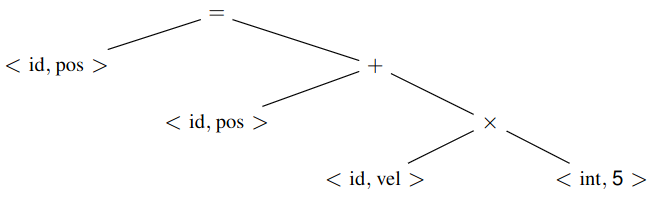
\includegraphics[scale=0.35]{8}
\end{center}

\begin{center}
  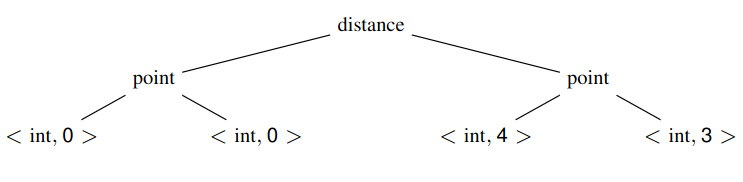
\includegraphics[scale=0.35]{9}
\end{center}

\begin{flushleft}
  \textbf{Nota:} Duas importantes características das árvores sintáticas são:

  \begin{enumerate}
    \item Não incluem alguns elementos lexicais (apenas relevantes para a sua estrutura formal);
    \item Definem, \textbf{sem ambiguidade}, a ordem das operações.
  \end{enumerate}
\end{flushleft}

\subsubsection{Análise Semântica}

\begin{flushleft}
  \item Parte final do "front end" do compilador.
  \item São verificadas todas as restantes restrições que não é possível, ou desejável, verificar nas fases anteriores.
  \item \textbf{Exemplo:} verificar se um identificador foi declarado,
  verificar a conformidade no sistema de tipos da
  linguagem, etc.
  \item Note-se que apenas restrições com verificação estática
  (i.e. em tempo de compilação), podem ser objeto de
  análise semântica pelo compilador.
  \item Se no exemplo 2 existisse a instrução de um círculo do
  qual fizesse parte a definição do seu raio, não seria em
  geral possível, durante a análise semântica, garantir um
  valor não negativo para esse raio (essa semântica apenas
  poderia ser verificada dinamicamente, i.e., em tempo de
  execução).
  \item Utiliza a árvore sintática da análise sintática assim
  como uma estrutura de dados designada por \textbf{tabela de
  símbolos} (assente em arrays associativos).
  \item Esta última fase de análise deve garantir o sucesso das
  fases subsequentes (geração e eventual optimização de
  código, ou interpretação).
\end{flushleft}

\subsubsection{Síntese}

\begin{flushleft}
  \item Havendo garantia de que o código da linguagem fonte é
  válido, então podemos passar aos efeitos pretendidos
  com esse código.
  \item Os efeitos podem ser:
  \begin{enumerate}
    \item simplesmente a indicação de validade do código fonte;
    \item a tradução do código fonte numa linguagem destino;
    \item ou a interpretação e execução imediata.
  \end{enumerate}
  \item Em todos os casos, pode haver interesse na identificação
  e localização precisa de eventuais erros.
  \item Como a maioria do código fonte assenta em texto, é usual
  indicar não só a instrução mas também a linha onde cada
  erro ocorre.
\end{flushleft}

\subsubsection{Geração de código: exemplo}

\begin{flushleft}
  \item Como dito antes, no processo de compilação, pode haver o interesse em
  gerar uma representação intermédia do código que facilite
  a geração final de código.
  \item Uma forma possível para essa representação intermédia
  é o chamado \textbf{código de triplo endereço}.
  \item Por exemplo para o exemplo 1 (\textbf{pos = pos + vel * 5;}):
  \begin{center}
    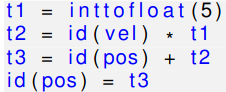
\includegraphics[scale=0.4]{10}
  \end{center}
  Este código poderia depois ser optimizado na fase
  seguinte da compilação:
  \begin{center}
    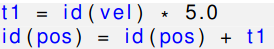
\includegraphics[scale=0.4]{11}
  \end{center}
  E por fim, poder-se-ia gerar assembly (pseudo-código):
  \begin{center}
    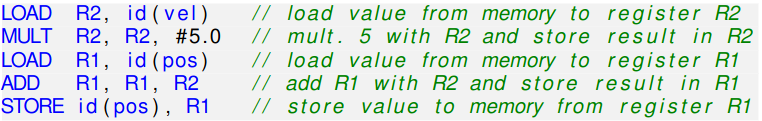
\includegraphics[scale=0.4]{12}
  \end{center}
\end{flushleft}

\pagebreak

\subsection{Linguagens: Definição como Conjunto}

\begin{flushleft}
  \item As linguagens servem para \textbf{comunicar}.
  \item Uma mensagem pode ser vista como uma sequência de
  \textbf{símbolos}.
  \item No entanto, uma linguagem não aceita todo o tipo de
  símbolos e de sequências
  \item Uma linguagem é caracterizada por um conjunto de
  símbolos e uma forma de descrever sequências válidas
  desses símbolos (i.e. o conjunto de sequências válidas).
  \item Se as linguagens naturais admitem alguma subjetividade
  e ambiguidade, as linguagens de programação requerem
  total objetividade.
  \item Como definir linguagens de forma sintética e objetiva?
  \item Definir por \textbf{extensão} é uma possibilidade.
  \item No entanto, para linguagens minimamente interessantes
  não só teríamos uma descrição gigantesca como
  também, provavelmente, incompleta.
  \item As linguagens de programação tendem a aceitar variantes
  infinitas de entradas.
  \item Alternativamente podemos descrevê-la por \textbf{compreensão}.
  \item Uma possibilidade é utilizar os formalismos ligados à
  definição de \textbf{conjuntos}.
\end{flushleft}

\subsection{Conceitos Básicos e Terminologia}

\begin{flushleft}
  \item Um conjunto pode ser definido por \textbf{extensão} (ou
  enumeração) ou por \textbf{compreensão}.
  \item Um exemplo de um conjunto definido por extensão é o
  conjunto dos algarismos binários \{0, 1\}.
  \item Na definição por compreensão utiliza-se a seguinte
  notação: \textbf{$\{x \hspace{1mm}| \hspace{1mm} p(x)\}$ ou $\{x \hspace{1mm}: \hspace{1mm} p(x)\}$}
  \item $x$ é a variável que representa um qualquer elemento do
  conjunto, e $p(x)$ um predicado sobre essa variável.
  \item Assim, este conjunto é definido contendo todos os valores
  de $x$ em que o predicado $p(x)$ é verdadeiro.
  \item \textbf{Exemplo:} $\{ n \hspace{1mm} | \hspace{1mm} n \hspace{1mm} \in \hspace{1mm} \mathbb{N} \hspace{1mm} \wedge n \le 9 \} = \{1,2,3,4,5,6,7,8,9\} $
  \item \textbf{Símbolo} (ou \textbf{Letra} -) é a unidade atómica (indivisível)
  das linguagens.
  \item Em linguagens assentes em texto, um símbolo será um
  carácter.
  \item \textbf{Alfabeto -} é um conjunto finito não vazio de símbolos.
  \item \textbf{Exemplo:} $A = \{0, 1\}$ é o alfabeto dos algarismos binários.
  
  $A = \{0, 1, \dots, 9\}$ é o alfabeto dos algarismos decimais.

  \item \textbf{Palavra -} (string ou cadeia) é uma sequência de
  símbolos sobre um dado alfabeto A.

  $U = a_1 a_2 \dots a_n$, com $a_i \in A \hspace{1mm} \wedge n \ge 0$

  \item $A = \{0,1, \dots, 9\}$ é o alfabeto dos algarismos decimais.
  2016, 234523, 999999999999999, 0

  $A = \{0,1, \dots,0,a,b, \dots, z, @, \dots \}$ mos@ua.pt, Bom dia!

  \item \textbf{Palavra vazia}  é uma sequência de zero símbolos e
  denota-se por $\varepsilon $ (épsilon).
  \item Note que $\varepsilon$ não pertence ao alfabeto.
  \item Uma \textbf{Sub-palavra} de uma palavra u é uma sequência
  contígua de 0 ou mais símbolos de u.
  \item Um \textbf{Prefixo} de uma palavra u é uma sequência contígua
  de 0 ou mais símbolos iniciais de u.
  \item Um \textbf{Sufixo} de uma palavra u é uma sequência contígua de
  0 ou mais símbolos terminais de u.
  \item \textbf{Exemplo:}
  \begin{itemize}
    \item $as$ é uma sub-palavra de $casa$, mas não prefixo nem sufixo;
    \item $001$ é prefixo e sub-palavra de $00100111$ mas não é sufixo;
    \item $\varepsilon$ é prefixo, sufixo e sub-palavra de qualquer palavra u;
    \item qualquer palavra u é prefixo, sufixo e sub-palavra de si
    própria
  \end{itemize}
  \item O \textbf{Fecho (ou conjunto de cadeias)} do alfabeto A
  denominado por $A^*$, representa o conjunto de todas as
  palavras definíveis sobre o alfabeto A, incluindo a palavra
  vazia.
  \item \textbf{Exemplo:} $\{0,1\}^* = \{\varepsilon,0,1,00,01,10,11,000,001,\dots\}$
  \item Dado um alfabeto A, uma \textbf{linguagem} L sobre A é um
  conjunto finito ou infinito de palavras consideradas válidas
  definidas com símbolos de A (isto é $L \subseteq A^*$).
  \item \textbf{Exemplo} de linguagens sobre o alfabeto $A = \{0,1\}$:
  \begin{itemize}
    \item $L_1 = \{u \hspace{1mm} | \hspace{1mm} u \in A^* \wedge |u| \le 2\} = \{\varepsilon, 0,1,00,01,10,11\}$
    \item $L_2 = \{u \hspace{1mm} | \hspace{1mm} u \in A^* \wedge \forall_i \hspace{1mm} u_i = 0\} = \{\varepsilon, 0, 00, 000, 0000, \dots\}$
    \item $L_3 = \{u \hspace{1mm} | \hspace{1mm} u \in A^* \wedge u.count(1) \hspace{1mm} mod \hspace{1mm} 2 = 0\} = \{000,11,000110101,\dots\}$
    \item $L_4 = \{\} = \emptyset$ (conjunto vazio)
    \item $L_5 = \{\varepsilon\}$
    \item $L_6 = A$
    \item $L_7 = A^*$
  \end{itemize}
  \item Note que \{\}, \{$\varepsilon$\}, $A$, $A^*$, são linguagens sobre o alfabeto
  $A$ qualquer que seja $A$.
  \item Uma vez que as linguagens são conjuntos, todas as
  operações matemáticas sobre conjuntos são aplicáveis:
  reunião, intercepção, complemento, diferença, \dots
\end{flushleft}

\subsection{Operações sobre palavras}

\begin{flushleft}
  \item O \textbf{comprimento} de uma palavra $u$ denota-se por $| u |$ e
  representa o seu número de símbolos.
  \item O comprimento da palavra vazia é zero: $|\varepsilon| = 0$.
  \item É habitual interpretar-se a palavra u como uma função de
  acesso aos seus símbolos (tipo "array" de símbolos): $u : \{1,2,\dots,n\} \rightarrow A$, com $n = |u|$
  (em que $u_i$ representa o iésimo símbolo de $u$).
  \item O \textbf{reverso} de uma palavra $u$ é a palavra, denota-se por
  $u^R$ , e é obtida invertendo a ordem dos símbolos de $u$, $u = \{u_1,u_2,\dots,u_n\} \Longrightarrow u^R = \{u_n,\dots,u_2,u_1\}$
  \item A \textbf{concatenação (ou produto)} das palavras $u$ e $v$ denota-se por $u.v$,
  ou simplesmente $uv$, e representa a justaposição de $u$ e $v$, i.e, a palavra constituída pelos
  símbolos de $u$ seguidos pelos símbolos de $v$.
  \item Propriedades da concatenação:
  \begin{itemize}
    \item $|u.v| = |u| + |v|$
    \item $u.(v.w) = (u.v).w = u.v.w$ (associatividade)
    \item $u.\varepsilon = \varepsilon.u = u$ (elemento neutro)
    \item $u \ne \varepsilon \wedge v \ne \varepsilon \wedge u \ne v \Longrightarrow u.v \ne v.u$ (não comutativo)
  \end{itemize}
  \item A \textbf{potência} de ordem $n$, com $n \le 0$, de uma palavra $u$ denota-se
  por um $u^n$ e representa a concatenação de $n$ réplicas de $u$, ou seja, $\underbrace{uu\dots u}_\text{nx}$
  \item $u^0 = \varepsilon$
\end{flushleft}

\subsection{Operações sobre linguagens}

\subsubsection{Reunião}

\begin{flushleft}
  \item Denota-se por: $L_1 \cup L_2$ e é dada por: $L_1 \cup L_2 = \{u \hspace{1mm} | \hspace{1mm} u \in L_1 \vee u \in L_2 \}$
  \item Se definirmos as linguagens $L_1$ e $L_2$ sobre o alfabeto $A = \{a,b\}$:
  \begin{itemize}
    \item $L_1 = \{u \hspace{1mm} | \hspace{1mm} u$ começa por $a\} = \{a w \hspace{1mm} | \hspace{1mm} w \in A^*\}$
    \item $L_2 = \{u \hspace{1mm} | \hspace{1mm} u$ termina por $a\} = \{w a \hspace{1mm} | \hspace{1mm} w \in A^*\}$
  \end{itemize}
  \item $L_1 \cup L_2 = \{w_1 \hspace{1mm} a \hspace{1mm} w_2 \hspace{1mm} | \hspace{1mm}, w_1,w_2 \in A^* \wedge (w_1 = \varepsilon \vee w_2 = \varepsilon)\}$
\end{flushleft}

\subsubsection{Interceção}

\begin{flushleft}
  \item Denota-se por: $L_1 \cap L_2$ e é dada por: $\{u \hspace{1mm} | \hspace{1mm} u \in L_1 \wedge u \in L_2\}$
  \item Usando o mesmo exemplo de cima: $L_1 \cap L_2 = \{a \hspace{1mm} w \hspace{1mm} a \hspace{1mm} | \hspace{1mm} w \in A^*\} \cup \{a\}$

  (esta última parte é necessário pois mesmo que $w = \varepsilon$, $a$ seria seguido por outro, $aa$)

\end{flushleft}

\subsubsection{Diferença}

\begin{flushleft}
  \item Denota-se por: $L_1 - L_2$ e é dada por: $\{u \hspace{1mm} | \hspace{1mm} u \in L_1 \wedge u \notin L_2\}$
  \item Usando o mesmo exemplo de cima: $L_1 - L_2 = \{a \hspace{1mm} w \hspace{1mm} x \hspace{1mm} | \hspace{1mm} w \in A^* \wedge x \in A \wedge x \ne a\}$
  
  \textbf{ou}

  $L_1 - L_2 = \{a \hspace{1mm} w \hspace{1mm} b \hspace{1mm} | \hspace{1mm} w \in A^*\}$
\end{flushleft}

\subsubsection{Complementação}

\begin{flushleft}
  \item Denota-se por: $\overline{L}$ e é dada por: $A^* - L = \{u \hspace{1mm} | \hspace{1mm} u \notin L \}$
  \item Usando o mesmo exemplo de cima: $\overline{L_1} = \{x \hspace{1mm} w \hspace{1mm} | \hspace{1mm} w \in A^* \wedge x \in A \wedge x \ne a\} \cup \{\varepsilon\}$
  
  \textbf{ou}

  $\overline{L_1} = \{b \hspace{1mm} w \hspace{1mm} | \hspace{1mm} w \in A^*\} \cup \{\varepsilon\}$
\end{flushleft}

\subsubsection{Concatenação}

\begin{flushleft}
  \item Denota-se por: $L_1.L_2$ e é dada por: $\{u v \hspace{1mm} | \hspace{1mm} u \in L_1 \wedge v \in L_2\}$
  \item Usando o mesmo exemplo de cima: $L_1.L_2 = \{a \hspace{1mm} w \hspace{1mm} a \hspace{1mm} | \hspace{1mm} w \in A^*\}$
\end{flushleft}

\subsubsection{Potenciação}

\begin{flushleft}
  \item Denota-se por: $L^n$ e é dada individualmente por:
  
  $\begin{cases}
    L^0 = \{\varepsilon\}\\
    L^{n+1} = L^n.L
  \end{cases}$
  \item Usando o mesmo exemplo de cima: $L_1^2= \{a \hspace{1mm} w_1 \hspace{1mm} a \hspace{1mm} w_2 \hspace{1mm} | \hspace{1mm} w_1, w_2 \in A^*\}$
\end{flushleft}

\subsubsection{Fecho de Kleene}

\begin{flushleft}
  \item Denota-se por: $L^*$ e é dado por: \[L^0 \cup L^1 \cup L^2 \cup \dots = \bigcup_{i = 0}^\infty  L^i\]
  \item Usando o mesmo exemplo de cima: $L_1^* = L_1 \cup \{\varepsilon\}$
  \item Note que para $n > 1$ $L_1^n \subset L_1$
\end{flushleft}

\subsubsection{Notas adicionais}

\begin{flushleft}
  \item Note que nas operações binárias sobre conjuntos não é
  requerido que as duas linguagens estejam definidos sobre
  o mesmo alfabeto.
  \item Assim se tivermos duas linguagens $L_1$ e $L_2$ definidas
  respetivamente sobre os alfebetos $A_1$ e $A_2$, então o
  alfabeto resultante da aplicação duma qualquer operação
  binária sobre as linguagens é: $A_1 \cup A_2$
\end{flushleft}

\pagebreak

\subsection{Introdução às gramáticas}

\subsubsection{Gramáticas}

\begin{flushleft}
  \item A utilização de conjuntos para definir linguagens não é
  frequentemente a forma mais adequada e versátil para as
  descrever.
  \item Muitas vezes é preferível identificar estruturas
  intermédias, que abstraem partes ou subconjuntos
  importantes, da linguagem.
  \item Tal como em programação, muitas vezes descrições
  recursivas são bem mais simples, sem perda da
  objetividade e do rigor necessários.
  \item É nesse caminho que encontramos as \textbf{gramáticas}.
  \item As \textbf{gramáticas} descrevem linguagens por compreensão
  recorrendo a representações \textbf{formais} e (muitas vezes)
  \textbf{recursivas}.
  \item Vendo as linguagens como sequências de símbolos (ou
  palavras), as gramáticas definem formalmente as
  sequências \textbf{válidas}.
\end{flushleft}

\begin{flushleft}
  \textbf{Exemplo:} Em português a frase "O cão ladra" pode ser gramaticalmente descrita por:
  \begin{center}
    \item frase $\rightarrow$ sujeito predicado
    \item sujeito $\rightarrow$ artigo substantivo
    \item predicado $\rightarrow$ verbo
    \item artigo $\rightarrow$ \textbf{O $|$ Um}
    \item substantivo $\rightarrow$ \textbf{cão $|$ lobo}
    \item verbo $\rightarrow$ \textbf{ladra $|$ uiva}
  \end{center}
  \item Esta gramática descreve 8 possíveis frases e contém mais
  informação do que a frase original.
  \item Contém 6 \textbf{símbolos terminais} e 6 \textbf{símbolos não terminais}.
  \item Um símbolo não terminal é definido por uma \textbf{produção}
  descrevendo possíveis representações desse símbolo, em
  função de símbolos terminais e/ou não terminais.
\end{flushleft}

Formalmente, uma gramática é um quádruplo G = (T , N, S, P), onde:
\begin{enumerate}
  \item $T$ é um conjunto finito não vazio designado por alfabeto
  terminal, onde cada elemento é designado por \textbf{símbolo
  terminal};
  \item $N$ é um conjunto finito não vazio, disjunto de $T (N \cap T = \emptyset)$,
  cujos elementos são designados por \textbf{símbolos não
  terminais};
  \item $S \in N$ é um símbolo não terminal específico designado por
  \textbf{símbolo inicial};
  \item $P$ é um conjunto finito de \textbf{regras} (ou \textbf{produções}) da forma:
  
  $\alpha \rightarrow \beta$ onde $\alpha \in (T \cup N)^* N(T \cup N)^*$ e $\beta \in (T \cup N)^*$,
  isto é, $\alpha$ é uma cadeia de símbolos terminais e não terminais
  contendo, pelo menos, um símbolo não terminal e $\beta$ é uma
  cadeia de símbolos, eventualmente vazia, terminais e não
  terminais.
\end{enumerate}

\pagebreak

\begin{flushleft}
  \textbf{Exemplos:} Formalmente, a gramática anterior será:\break

  G = (\{\textbf{O, Um, cão, lobo, ladra, uiva}\}, \{frase, sujeito, predicado, artigo, substantivo, verbo\},
  frase, P)\break

  Em que P é constituído pelas regras já apresentadas (frase $\rightarrow$ sujeito predicado, \dots)\break

  Podemos descrever a frase “O cão ladra” com a seguinte
  árvore (denominada sintática).

  \begin{center}
    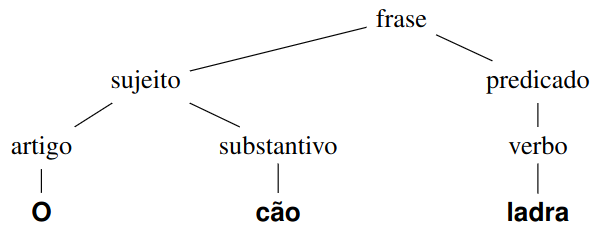
\includegraphics[scale=0.3]{13}
  \end{center}
\end{flushleft}

\begin{flushleft}
  Considere a seguinte gramática G = (\{0, 1\}, \{S, A\}, S, P), onde P é constituído pelas
  regras:

  \begin{center}
    \begin{tabular}{l}
      S $\rightarrow$ 0 S\\
      S $\rightarrow$ 0 A\\
      A $\rightarrow$ 0 A 1\\
      A $\rightarrow$ $\varepsilon$\\
    \end{tabular}
  \end{center}

  Qual será a linguagem definida por esta gramática?

  \[L = \{0^n 1^m : n \in \mathbb{N} \wedge m \in \mathbb{N}_0 \wedge n > m\}\]
\end{flushleft}

\subsection{Hierarquia de Chomsky}

\begin{flushleft}
  \item Restrições sobre $\alpha $e $\beta$ permitem definir uma taxonomia
  das linguagens - hierarquia de Chomsky:
  \begin{enumerate}
    \item Se não houver nenhuma restrição, G é designada por
    gramática do \textbf{tipo-0}.
    \item G será do \textbf{tipo-1}, ou gramática \textbf{dependente do contexto}, se
    se cada regra $\alpha \rightarrow \beta$ de P obedece a $| \alpha | \le | \beta |$ (com a
    excepção de também poder existir a produção vazia: $S \rightarrow \varepsilon$)
    \item G será do \textbf{tipo-2}, ou gramática \textbf{independente, ou livre, do
    contexto}, se cada regra $\alpha \rightarrow \beta$ de P obedece a $| \alpha | = 1$,
    isto é: $\alpha$ é constituído por um só não terminal.
    \item G será do \textbf{tipo-3}, ou gramática \textbf{regular}, se cada regra tiver
    uma das formas: $A \rightarrow c B$, $A \rightarrow c$ ou $A \rightarrow \varepsilon$, onde A e B
    são símbolos não terminais (A pode ser igual a B) e c um
    símbolo terminal. Isto é, em todas as produções, o $\beta$ só
    pode ter no máximo um símbolo não terminal sempre à
    direita (ou, alternativamente, sempre à esquerda)
  \end{enumerate}

  \begin{center}
    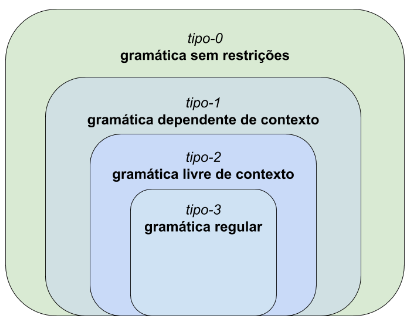
\includegraphics[scale=0.45]{14}
  \end{center}

  \item Para cada um desses tipos podem ser definidos diferentes
  tipos de máquinas (algoritmos, autómatos) que as podem
  reconhecer.
  \item Quanto mais simples for a gramática, mas simples e
  eficiente é a máquina que reconhece essas linguagens.
\end{flushleft}

\begin{flushleft}
  \item Cada classe de linguagens do \textbf{tipo-i} contém a classe de
  linguagens \textbf{tipo-(i +1)} (i = 0, 1, 2)
  \item Esta hierarquia não traduz apenas as características
  formais das linguagens, mas também expressam os
  requisitos de computação necessários:
  \begin{enumerate}
    \item As \textbf{máquinas de Turing} processam gramáticas sem
    restrições (tipo-0);
    \item Os \textbf{autómatos linearmente} limitados processam gramáticas
    dependentes do contexto (tipo-1);
    \item Os \textbf{autómatos de pilha} processam gramáticas
    independentes do contexto (tipo-2);
    \item Os \textbf{autómatos finitos} processam gramáticas regulares
    (tipo-3).
  \end{enumerate}
\end{flushleft}

\subsection{Autómatos}

\subsubsection{Máquina de Turing}

\begin{flushleft}
  \item (Alan Turing, 1936)
  \item Modelo abstrato de computação.
  \item Permite (em teoria) implementar qualquer programa
  computável.
  \item Assenta numa máquina de estados finita, numa "cabeça"
  de leitura/escrita de símbolos e numa fita infinita (onde se
  escreve ou lê esses símbolos).
  \item A "cabeça" de leitura/escrita pode movimentar-se uma
  posição para esquerda ou direita.
  \item Modelo muito importante na teoria da computação.
  \item Pouco relevante na implementação prática de
  processadores de linguagens.
\end{flushleft}

\begin{center}
  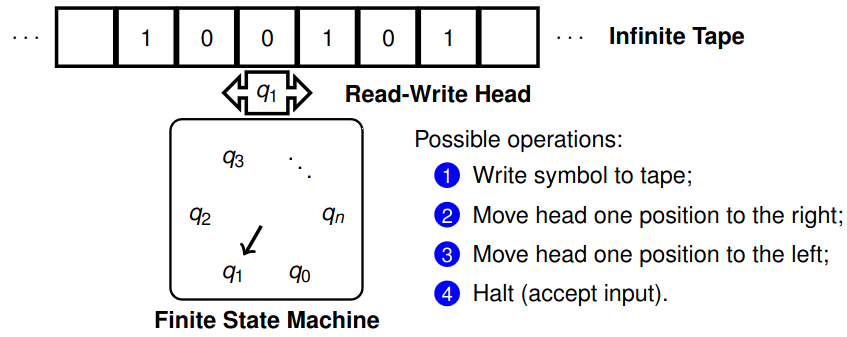
\includegraphics[scale=0.35]{15}
\end{center}

\begin{flushleft}
  \item A máquina de estados finita (FSM) tem acesso ao símbolo
  atual e decide a próxima ação a ser realizada.
  \item A ação consiste na transição de estado e qual a
  operação sobre a fita.
  \item Se não for possível nenhuma acção, a entrada é rejeitada.
\end{flushleft}

\begin{flushleft}
  \textbf{Exemplo}
\end{flushleft}

\begin{flushleft}
  \item Dado o alfabeto A = \{0, 1\}, e considerando que um
  número inteiro não negativo n é representado pela
  sequência de n + 1 símbolos 1, vamos implementar uma
  MT que some os próximos (i.e à direita da posição actual)
  dois números inteiros existentes na fita (separados
  apenas por um 0).
  \item O algoritmo pode ser simplesmente trocar o símbolo 0
  entre os dois números por 1, e trocar os dois últimos
  símbolos 1 por 0.
  \item Por exemplo: 3 + 2 a que corresponde o seguinte estado
  na fita (símbolo a negrito é a posição da "cabeça"):

  · · · \textbf{0}111101110 · · · (o resultado pretendido será:

  · · · \textbf{0}111111000 · · · ).\break

  Considerando que os estados são designados por
  $E_i$ , $i$ $\ge$ 1 (sendo $E_1$ o estado inicial); e as operações:
  \begin{itemize}
    \item \textbf{d} mover uma posição para a direita;
    \item \textbf{e} mover uma posição para a esquerda;
    \item \textbf{0} escrever o símbolo 0 na fita;
    \item \textbf{1} escrever o símbolo 1 na fita;
    \item \textbf{h} aceitar e terminar autómato.
  \end{itemize}
\end{flushleft}

\pagebreak

\begin{flushleft}
  Uma solução possível é dada pela seguinte diagrama de
  transição de estados:

  \begin{center}
    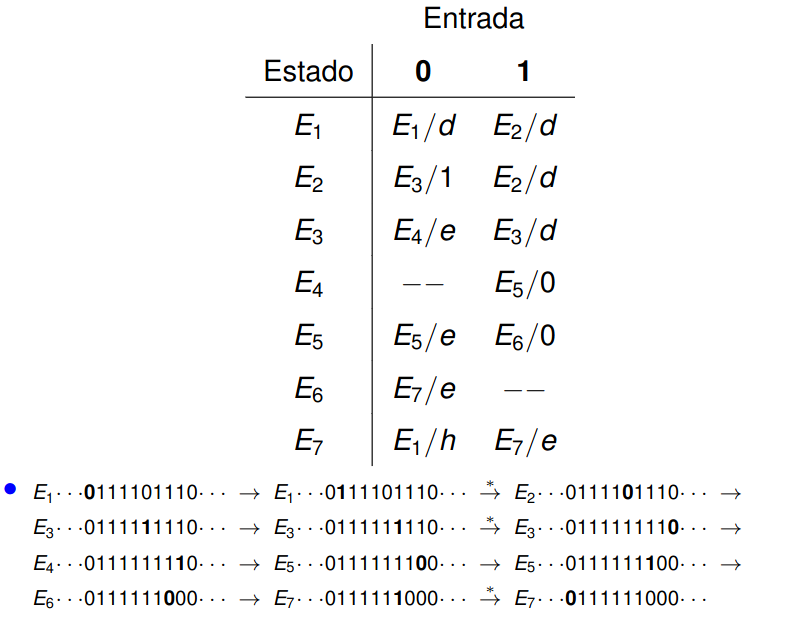
\includegraphics[scale=0.35]{16}
  \end{center}
\end{flushleft}

\subsubsection{Autómatos linearmente limitados}

\begin{flushleft}
  Diferem das MT pela finitude da fita.

  \begin{center}
    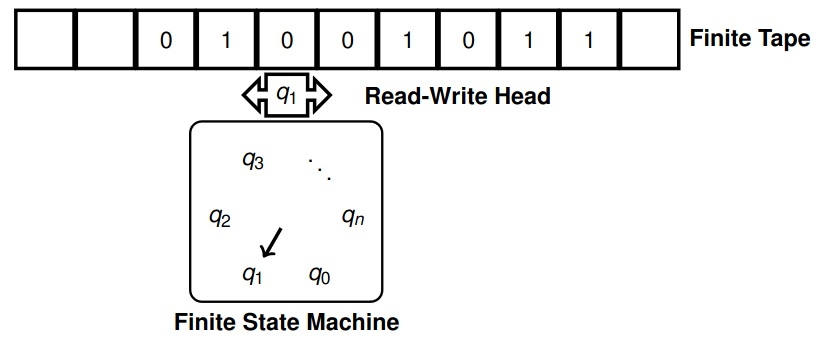
\includegraphics[scale=0.35]{17}
  \end{center}
\end{flushleft}

\pagebreak

\subsubsection{Autómatos de pilha}

\begin{flushleft}
  \item "Cabeça" apenas de leitura e suporte de uma pilha sem
  limites.
  \item Movimento da "cabeça" apenas numa direção.
  \item Autómatos adequados para análise sintática.

  \begin{center}
    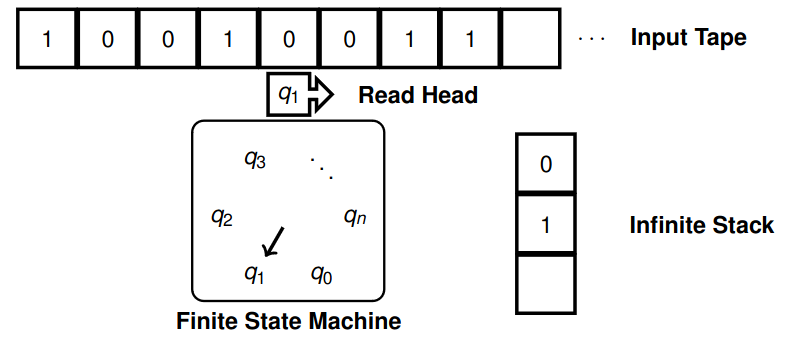
\includegraphics[scale=0.35]{18}
  \end{center}
\end{flushleft}

\subsubsection{Autómatos finitos}

\begin{flushleft}
  \item Sem escrita de apoio à máquina de estados.
  \item Autómatos adequados para análise léxica.

  \begin{center}
    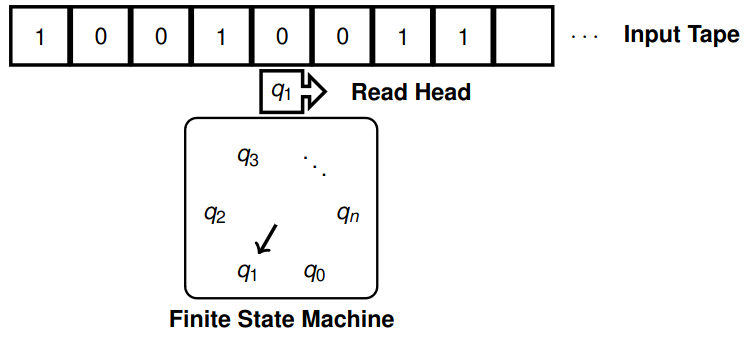
\includegraphics[scale=0.35]{19}
  \end{center}
\end{flushleft}

\pagebreak

\section{Tema 2 - ANTLR4}

\begin{flushleft}
  \textbf{ANTLR4 -} \textbf{AN}other\textbf{ T}ool for \textbf{L}anguage \textbf{R}ecognition é um gerador de processadores de
  linguagens que pode ser usado para ler, processar, executar ou traduzir linguagens.
\end{flushleft}

\subsection{Exemplos Introdutórios}

\begin{center}
  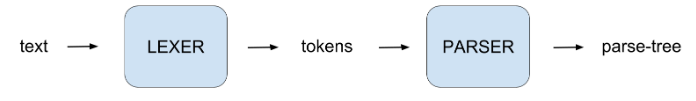
\includegraphics[scale=0.35]{20}
\end{center}

\begin{flushleft}
  \textbf{Exemplo Hello:}
\end{flushleft}

\begin{center}
  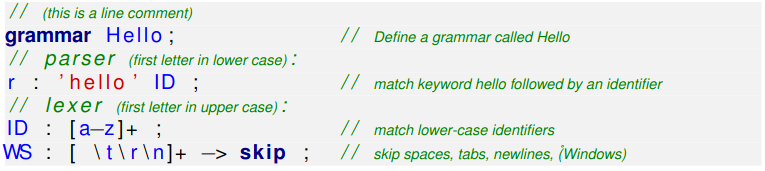
\includegraphics[scale=0.35]{21}
\end{center}

\begin{flushleft}
  \item As duas gramáticas - lexical e sintática - são expressas com instruções em a
  seguinte estrutura: $\alpha : \beta;$
  \item Em que $\alpha$ corresponde a um único símbolo lexical ou sintático (dependendo dada
  sua primeira letra ser, respetivamente, maiúscula ou minúscula); e em que $\beta$
  é uma expressão simbólica equivalente a $\alpha$.

  \item \textbf{Parser -} Composição de Tokens numa estrutura sintática adequada.
  \item \textbf{Lexer -} Composição de letras e outros caracteres em palavras (Tokens).
\end{flushleft}

\begin{flushleft}
  \item Uma sequência de símbolos na entrada que seja
  reconhecido por esta regra gramatical pode sempre ser
  expressa por uma estrutura tipo árvore (chamada
  sintática), em que a raiz corresponde a $\alpha$ e os ramos à
  sequência de símbolos expressos em $\beta$:

  \begin{center}
    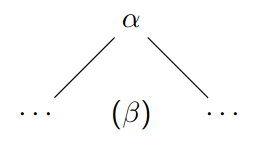
\includegraphics[scale=0.3]{22}
  \end{center}

  \item Executando o comando \uline{antlr4} sobre a gramática \uline{Hello.g4} temos:
  
  \begin{center}
    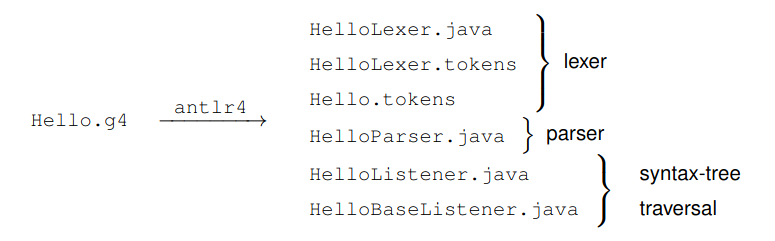
\includegraphics[scale=0.4]{23}
  \end{center}


  \pagebreak

  \item Ficheiros gerados:
  \begin{itemize}
    \item \textbf{HelloLexer.java}: código \textbf{Java} com a análise léxica
    (gera tokens para a análise sintática);
    \item \textbf{Hello.tokens} e \textbf{HelloLexer.tokens}: ficheiros com a
    identificação de tokens (pouco importante nesta fase, mas
    serve para modularizar diferentes analisadores léxicos e/ou
    separar a análise léxica da análise sintática);
    \item \textbf{HelloParser.java}: código \textbf{Java} com a análise
    sintática (gera a árvore sintática do programa);
    \item \textbf{HelloListener.java} e \textbf{HelloBaseListener.java}:
    código \textbf{Java} que implementa automaticamente um padrão
    de execução de código tipo listener (observer, callbacks)
    em todos os pontos de entrada e saída de todas as regras
    sintáticas do compilador.
  \end{itemize}

  \item Podemos executar o \textbf{ANTLR4} com a opção \textbf{-visitor}
  para gerar também código \textbf{Java} para o padrão tipo visitor
  (difere do listener porque a visita tem de ser
  explicitamente requerida).
  \item \textbf{HelloVisitor.java} e \textbf{HelloBaseVisitor.java}:
  código \textbf{Java} que implementa automaticamente um padrão
  de execução de código tipo visitor todos os pontos de
  entrada e saída de todas as regras sintáticas do
  compilador.

\end{flushleft}

\begin{flushleft}
  \textbf{Exemplo Expr}

  \begin{center}
    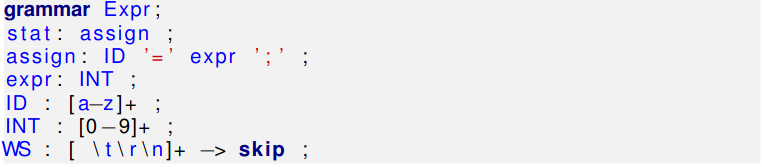
\includegraphics[scale=0.35]{24}
  \end{center}

  \item Se executarmos o compilador criado com a entrada:
  \[\textbf{sp} = 100;\]
  \item Vamos obter a seguinte árvore sintática:
  
  \begin{center}
    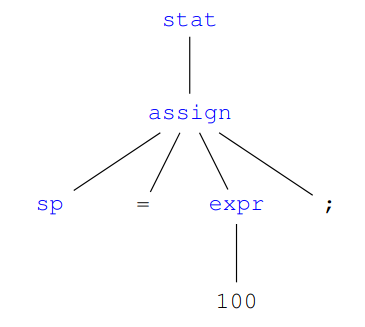
\includegraphics[scale=0.4]{25}
  \end{center}

  \item Para facilitar a análise semântica e a síntese, o \textbf{ANTLR4}
  tenta ajudar na resolução automática de muitos
  problemas (como é o caso dos visitors e dos listeners).
  \item No mesmo sentido são geradas classes (e em execução
  os respetivos objetos) com o contexto de todas as
  regras da gramática:

  \begin{center}
    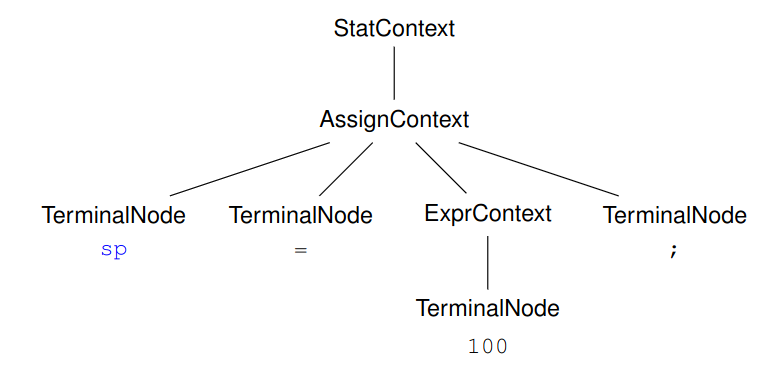
\includegraphics[scale=0.35]{26}
  \end{center}


  \begin{center}
    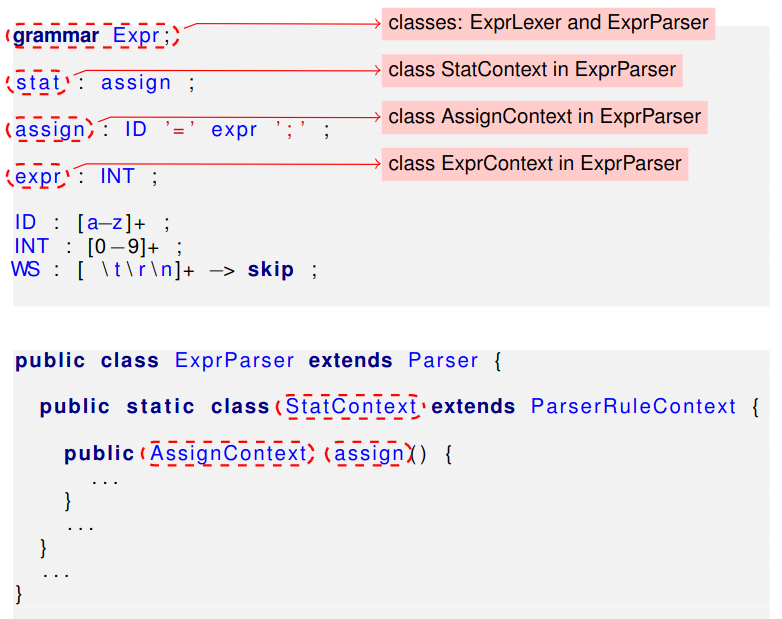
\includegraphics[scale=0.3]{27}
  \end{center}
\end{flushleft}

\subsubsection{Visitor}

\begin{flushleft}
  \item Os objetos de contexto têm a si associada toda a
  informação relevante da análise sintática (tokens,
  referência aos nós filhos da árvore, etc.)
  \item Por exemplo o contexto \textbf{AssignContext} contém
  métodos \textbf{ID} e \textbf{expr} para aceder aos respetivos nós.

  \pagebreak
  \item No caso do código gerado automaticamente do tipo visitor
  o padrão de invocação é ilustrado a seguir:

  \begin{center}
    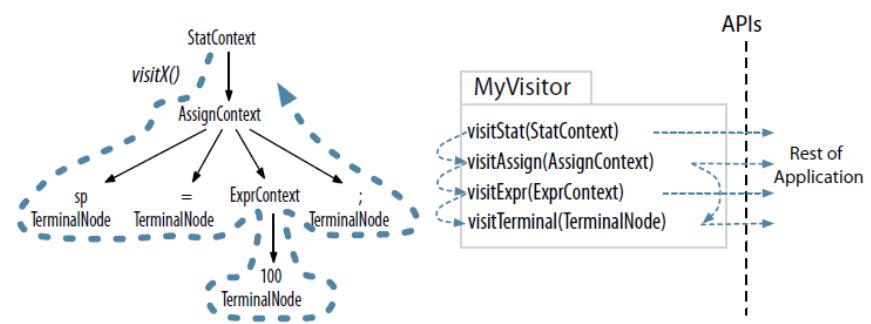
\includegraphics[scale=0.3]{28}
  \end{center}
\end{flushleft}

\subsubsection{Listener}

\begin{flushleft}
  \item  O código gerado automaticamente do tipo listener tem o
  seguinte padrão de invocação (ordem de execução):

  \begin{center}
    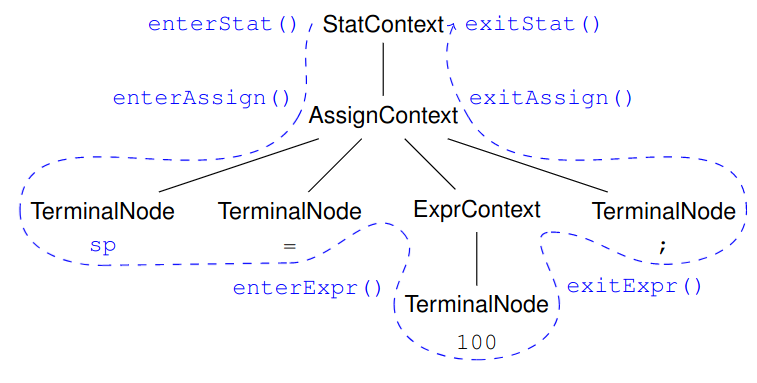
\includegraphics[scale=0.3]{29}
  \end{center}

  \item A sua ligação à restante aplicação é a seguinte:

  \begin{center}
    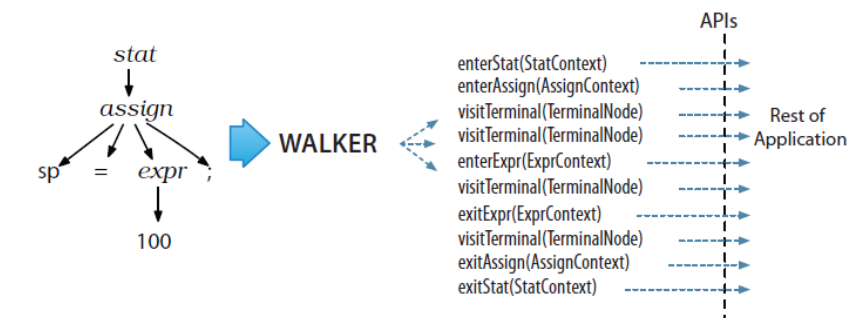
\includegraphics[scale=0.3]{30}
  \end{center}
\end{flushleft}

\pagebreak
\subsubsection{Atributos e ações}

\begin{flushleft}
  \item É possível associar atributos e ações às regras:

  \begin{center}
    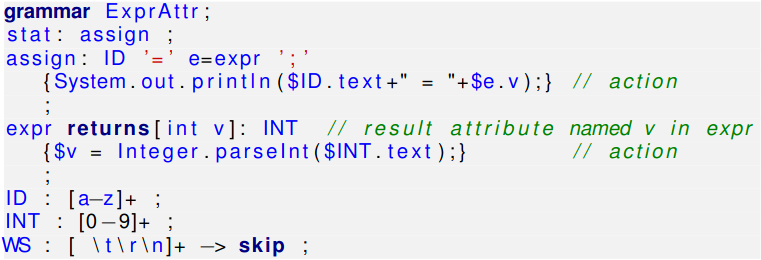
\includegraphics[scale=0.3]{31}
  \end{center}

  \item Ao contrário dos visitors e listeners, a execução das
  ações ocorre durante a análise sintática.
  \item A execução de cada ação ocorre no contexto onde ela é
  declarada. Assim se uma ação estiver no fim de uma
  regra (como exemplificado acima), a sua execução
  ocorrerá após o respetivo reconhecimento.
  \item A linguagem a ser executada na ação não tem de ser
  necessariamente Java (existem muitas outras possíveis,
  como C++ e python).
  \item Também podemos passar atributos para a regra (tipo
  passagem de argumentos para um método):

  \begin{center}
    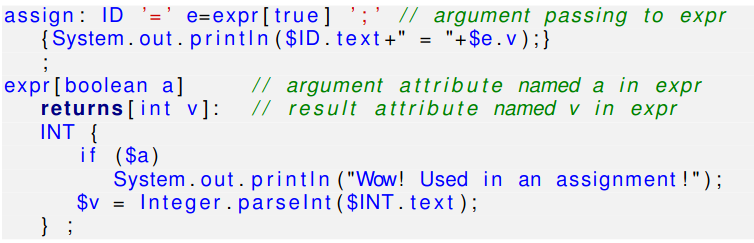
\includegraphics[scale=0.3]{32}
  \end{center}

  \item É clara a semelhança com a passagem de argumentos e
  resultados de métodos.
  \item Diz que os atributos são \textbf{sintetizados} quando a informação
  provém de sub-regras, e \textbf{herdados} quando se envia
  informação para sub-regras.
\end{flushleft}

\subsection{Construção de gramáticas}

\begin{flushleft}
  \item A construção de gramáticas pode ser considerada uma
  forma de programação simbólica, em que existem
  símbolos que são equivalentes a sequências (que façam
  sentido) de outros símbolos (ou mesmo dos próprios).
  \item Os símbolos utilizados dividem-se em \textbf{símbolos terminais
  e não terminais}.
  \item Os símbolos terminais correspondem a caracteres na
  gramática lexical e tokens na sintática; e os símbolos não
  terminais são definidos por produções (regras).
  \item No fim, todos os símbolos não terminais devem poder ser
  expressos em símbolos terminais.
  \item Uma gramática é construída especificando as \textbf{regras} ou
  produções dos elementos gramaticais.

  \begin{center}
    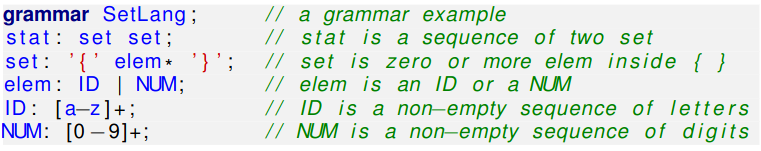
\includegraphics[scale=0.3]{33}
  \end{center}

  \item Sendo a sua construção uma forma de programação,
  podemos beneficiar da identificação e reutilização de
  padrões comuns de resolução de problemas.
  \item Surpreendentemente, o número de padrões base é
  relativamente baixo:
  \begin{itemize}
    \item \textbf{Sequência:} sequência de elementos;
    \item \textbf{Optativo:} aplicação optativa do elemento (zero ou uma
    ocorrência);
    \item \textbf{Repetitivo:} aplicação repetida do elemento (zero ou mais,
    uma ou mais);
    \item \textbf{Alternativa:} escolha entre diferentes alternativas (como por
    exemplo, diferentes tipos de instruções);
    \item \textbf{Recursão:} definição direta ou indiretamente recursiva de
    um elemento (por exemplo, instrução condicional é uma
    instrução que selecciona para execução outras instruções);
  \end{itemize}

  \item \textbf{Nota:} A recursão e a iteração são alternativas
  entre si. Admitindo a existência da sequência vazia, os
  padrões optativo e repetitivo são implementáveis com
  recursão.
  \item No entanto, como em programação em geral, por vezes é
  mais adequado expressar recursão, e outras iteração.
\end{flushleft}

\begin{flushleft}
  \textbf{Exemplo:}

  \begin{center}
    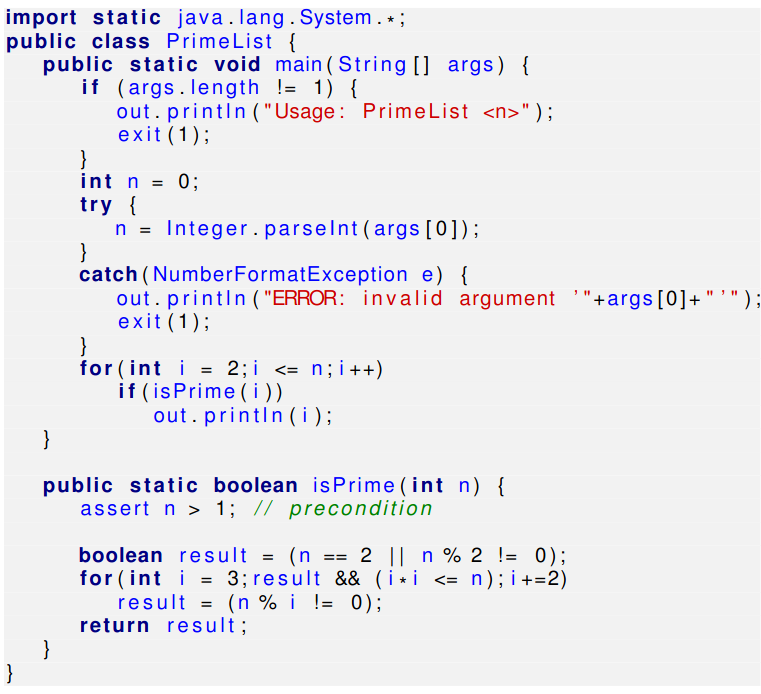
\includegraphics[scale=0.35]{34}
  \end{center}
\end{flushleft}

\pagebreak

\begin{flushleft}
  \item Mesmo sem uma gramática definida explicitamente,
  podemos neste programa inferir todos os padrões atrás
  referidos:
  \begin{itemize}
    \item \textbf{Sequência:} a instrução atribuição de valor é definida como
    sendo um identificador, seguido do carácter =, seguido de
    uma expressão.
    \item \textbf{Optativo:} a instrução condicional pode ter, ou não, a
    seleção de código para a condição falsa.
    \item \textbf{Repetitivo:} (1) uma classe é uma repetição de membros;
    (2) um algoritmo é uma repetição de comandos.
    \item \textbf{Alternativa:} diferentes instruções podem ser utilizadas onde
    uma instrução é esperada.
    \item \textbf{Recursão:} diferentes instruções podem ser utilizadas onde
    uma instrução é esperada.
  \end{itemize}
\end{flushleft}

\subsubsection{Especificação de gramáticas}

\begin{flushleft}
  \item Uma linguagem para especificação de gramáticas precisa
  de suportar este conjunto de padrões.
  \item Para especificar elementos léxicos (tokens) a notação
  utilizada assenta em expressões regulares.
  \item A notação tradicionalmente utilizada para a análise
  sintáctica denomina-se por BNF (Backus-Naur Form):
  \[<symbol> \textbf{::=} <meaning>\]
  \item Esta última notação teve origem na construção da
  linguagem Algol (1960).
  \item O ANTLR4 utiliza uma variação alterada e aumentada
  (Extended BNF ou EBNF) desta notação onde se pode
  definir construções opcionais e repetitivas.
  \[<symbol> \textbf{:} <meaning> ;\]
\end{flushleft}

\subsection{ANTLR4: Estrutura Léxica}




\end{document}